% ----------------------------------------------------------
\chapter{Modelo mecânico}
% ----------------------------------------------------------

Esse capítulo traz uma descrição geral do modelo mecânico que será utilizado neste trabalho. Portanto, são apresentadas as equações de equilíbrio e constitutivas que foram utilizadas, sem aprofundar, no entanto, nas particularidades que compreendem o domínio de um túnel profundo. Essas serão vistas no final do Capitulo 6, após a descrição da solução desse modelo mecânico. 

\section{Equações de Equilíbrio local e a hipótese da evolução quase estática}

A segunda lei fundamental do equilíbrio dinâmico, ou seja, o princípio da conservação do momento linear, aplicada sobre um subdomínio contínuo $\Omega'$, exige que para $\forall \Omega' \subset \Omega$:

\begin{equation}
	\label{conservacao_momento_linear}
\int_{\Omega'}\rho(\underline\gamma-\underline f)d\Omega' = \int_{\partial\Omega'}\underline T dS
\end{equation}

sendo $\rho$ a densidade do domínio, $\underline\gamma$ o campo de acelerações referente às forças inerciais, $\underline f$ o campo de acelerações referente às forças de corpo (por exemplo, a gravidade) e $\underline T$ o vetor tensão que atua na superfície $dS$ contida na superfície $\partial\Omega'$ de $\Omega'$ (\autoref{subsistema_material}).
%
\begin{figure}[H]
	\begin{center}
		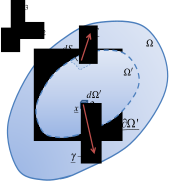
\includegraphics[scale = 1.0]{0501-subsistema no sistema material forças de corpo.pdf}
	\end{center}
	\caption{\label{subsistema_material}Subsistema material $\Omega'$ no interior de um sistema material $\Omega$ submetido a um campo de forças de corpo}
\end{figure}

Considerando a definição $\underline T = \underline{\underline\sigma}\cdot \underline n$ , em que $\underline n$ é o vetor normal à superfície $dS$ e $\underline{\underline\sigma}$ o tensor de tensões, aplicando o teorema da divergência no termo à direita da igualdade (\autoref{conservacao_momento_linear}) pode-se escrever que

\section{Admissibilidade estática, natureza Euleriana do Campo de Tensões, Transformação geométrica e medida de deformação}

\section{Hipótese das pequenas perturbações e a descrição Lagrangeana}

\section{Modelo constitutivo elástico}

\section{Modelo constitutivo elastoplástico}

\section{Modelo constitutivo viscoplástico}


\section{Modelo constitutivo elastoplástico-viscoplástico}







